\documentclass[notitlepage,longbibliography]{revtex4-1}

% Project name
\newcommand{\kms}{SmartKMS}

\usepackage{graphicx}
\usepackage{amsmath}
\usepackage[margin=5pt]{subfig}
\usepackage[usenames]{color}
\usepackage{librebaskerville}
% \usepackage{xspace}
\definecolor{darkgreen}{rgb}{0.00,0.50,0.25}
\definecolor{darkblue}{rgb}{0.00,0.00,0.67}
\newcommand{\figref}[1]{Fig.~\ref{#1}}
\usepackage[breaklinks,pdftitle={SmartKMS: blockchain-based encryption as a service}, pdfauthor={Michael Egorov},colorlinks,urlcolor=blue,citecolor=darkgreen,linkcolor=darkblue]{hyperref}
\usepackage[usenames]{color}
\graphicspath{{pdf/}}

\begin{document}

\title{\kms~--- blockchain-based key management as a service}

\author{M. Egorov}
\email{michael@nucypher.com}
\author{M. Wilkison}
\email{maclane@nucypher.com}
\affiliation{NuCypher}

% TODO: include David Nunez when he agrees

\begin{abstract}
    \kms~is a global, decentralized Key Management System.
    It provides encryption and cryptographic access controls as a service, performed by a decentralized network,
    with the help of proxy re-encryption~\cite{wiki:pre}.
    Importantly, it doesn't rely on trusting a service provider, unlike centralized encryption-as-a-service solutions.
    \kms~enables sharing of sensitive data for both decentralized and centralized applications,
    providing the infrastructure for applications from healthcare to identity to decentralized content marketplaces.
\end{abstract}

\date{\today}
\maketitle

\section{Introduction}

\kms~is a blockchain-based encryption and access control management as a service.
It enables secure private data sharing between arbitrary number of participants in public and/or decentralized networks.
Key Management Tokens (KMT) are used to perform key management and access delegation/revokation operations.

(Overview of encryption: symmetric encryption, public key encryption, encryption at rest, TLS).

(Overview of key management systems: what they do, why, KMS as a service - CloudHSM, truevault; self-run: hashicorp).

(Brief statement that we enable KMSaas with combination of blockchain and PRE)

\section{Architecture}

\subsection{Cryptographic primitives}

\subsubsection{Prior information and definitions}

Symmetric or secret key encryption requires users to know a common secret key.
We refer to this common secret key as DEK (data encryption key) for convenience.

Two operations are defined for symmetric ciphers:
$$c = \text{encrypt}_{sym}(dek, d),$$
$$d = \text{decrypt}_{sym}(dek, c),$$
where $d$ is plaintext data, and $c$ is ciphertext (encrypted data).

The most useful symmetric key encryption algorithms for our purposes are AES (because it's normally hardware-accelerated)~\cite{wiki:aes}
and Salsa20~\cite{wiki:salsa20}.

Symmetric block ciphers can operate in different modes.
We use modes of operation that yield probabilistic encryption (such as GCM for AES), which provide strong semantic security guarantees.
For simplicity, we omit details about the particular modes of operations, saying that the value of \emph{nonce} related to the mode of operation is a part of the
ciphertext $c$.

Public key encryption (PKE) is a type of encryption where two parties (a sender and receiver) exchange information without any required common secret.
Every participant has a key pair (a public $pk$ and a secret (or private) key $sk$).
If the sender has a key pair $sk_s/pk_s$ and the receiver~--- $sk_r/pk_r$, the sender can encrypt a message with the receiver's public key (which is known in advance),
and the receiver can decrypt with his secret key.

Hybrid cryptosystems can be created that combine the efficiency of symmetric encryption with the convenience of PKE.
An example hybrid cryptosytem encryption flow defines the functions:
$$dek = \text{random}();\qquad c = \text{encrypt}_{sym}(dek, d);\qquad edek=\text{encrypt}_{pke}(dek, pk_r).$$
The pair $(edek, c)$ is used to transfer the encrypted data.
The associated decryption by the receiver defines the functions:
$$dek=\text{decrypt}_{pke}(edek, sk_r);\qquad d = \text{decrypt}_{sym}(dek, c).$$

\subsubsection{Proxy re-encryption}
Proxy re-encryption (PRE)~\cite{wiki:pre,phd:nunez} is a type of public-key encryption (PKE) that allows a proxy entity to transform ciphertexts
from one public key to another, without learning anything about the underlying message~(Fig.~\ref{fig:pre}).

\begin{figure}
\centering
    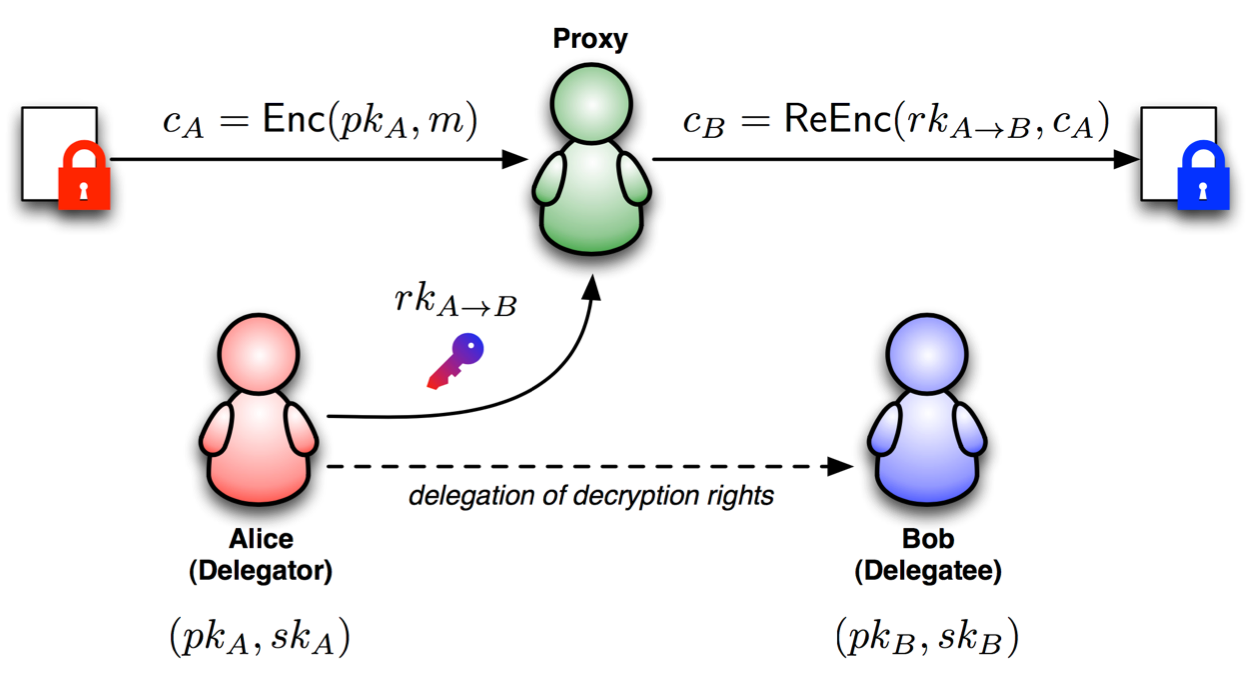
\includegraphics[width=0.6\columnwidth]{pdf/pre.png}  % XXX to be replaced with a vector re-draw
    \caption{Main actors and interactions in a PRE environment}
    \label{fig:pre}
\end{figure}

Alice, the data owner, encrypts a message $m$, with her public key $pk_A$, resulting in ciphertext $c_A$.
She decides to delegate access to message m to Bob who has the key pair $(pk_B, sk_B)$.
To do so, Alice creates a re-encryption key:
$$rk_{A\rightarrow B} = \text{rekey}(sk_A, pk_B).$$
Importantly, this re-encryption function is one way, and $rk_{A\rightarrow B}$ cannot be decomposed into its component parts
(at least, without knowing also $sk_A$ or $sk_B$).
All it can do is re-encrypt $c_A$ such that it is transformed into $c_B$:
$$c_B = \text{reencrypt}(rk_{A\rightarrow B}, c_{A}).$$
Bob can then decrypt $c_{B}$ using his secret key $sk_{B}$.

Compared to existing PKE protocols which are ideal for 1-to-1 communication, PRE is more scalable for N-to-N communication
with arbitrary numbers of producers and consumers.
It also doesn't require knowing the recipient of a message in advance, as the re-encryption tokens can be created and applied at any point.
This makes it well-suited for distributed systems such as blockchain, distributed networks, and big data~\cite{web:nucypher-hadoop}.

There are many proxy re-encryption algorithms, with different properties.
For the first version we choose the most simple one, derived from BBS98~\cite{BBS98}.
However, sometimes we want to delegate re-encryption to multiple nodes, in order to split the trust to apply time-based or conditional policy
between them.
In this case we use AFGH scheme~\cite{AFGH}.

\subsection{Re-encryption nodes}
\begin{figure}
\centering
    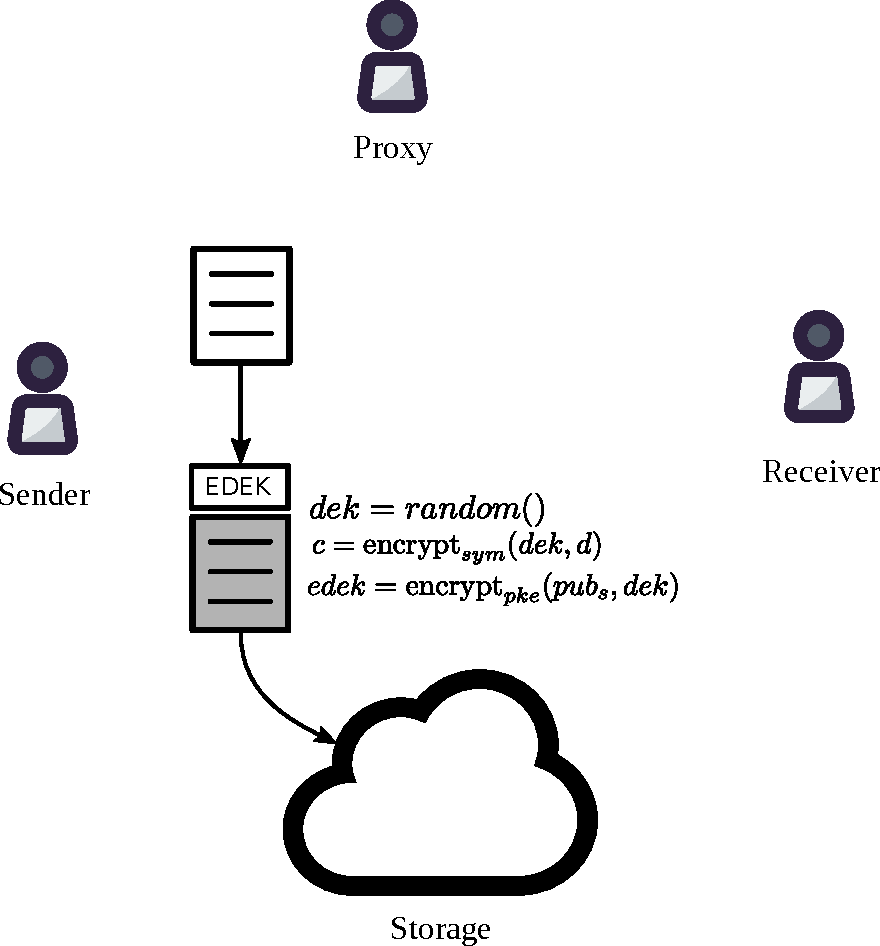
\includegraphics[width=0.4\columnwidth]{pdf/encrypt.pdf}
    \caption{Architecture: encryption}
    \label{fig:pre}
\end{figure}

\begin{figure}
\centering
    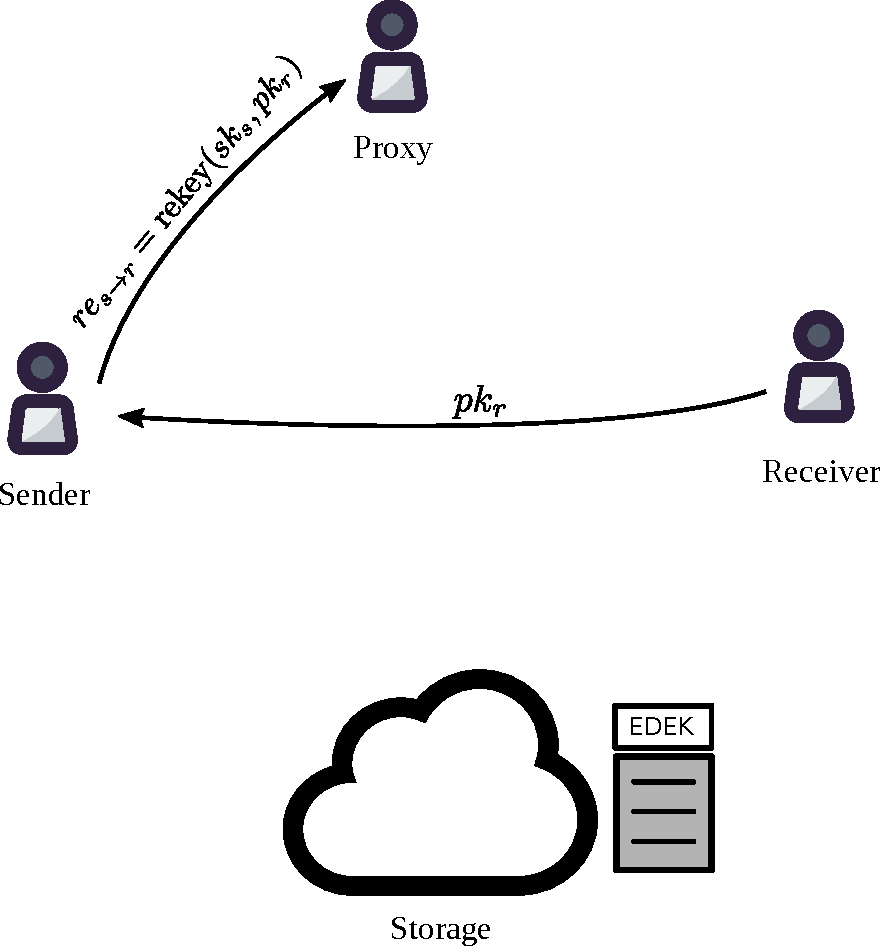
\includegraphics[width=0.4\columnwidth]{pdf/delegate.pdf}
    \caption{Architecture: access delegation}
    \label{fig:pre}
\end{figure}
\begin{figure}
\centering
    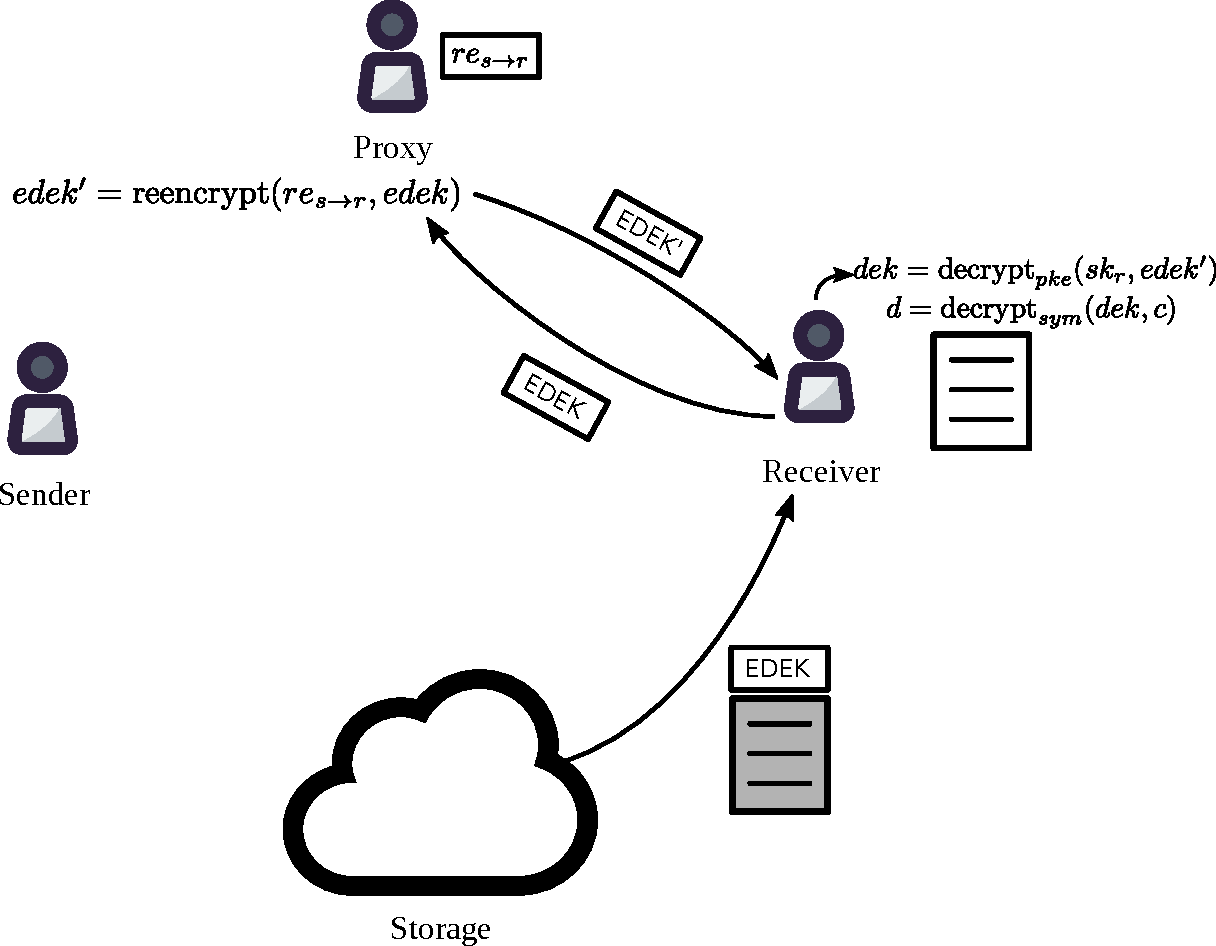
\includegraphics[width=0.6\columnwidth]{pdf/decrypt.pdf}
    \caption{Architecture: decryption}
    \label{fig:pre}
\end{figure}

\subsection{Local encryption library and daemon}

\section{Functionality}

\subsection{Sharing short secrets}

\subsection{Sharing files}

\subsection{Sharing encrypted streams}

\subsection{Time-based and condition-based policies}

\subsection{Policies controlled by smart contracts}

\subsection{Protocol extendibility}

\section{Economics}

\section{Use cases}
\kms~provides the infrastructure for a variety of applications that require sharing of sensitive data as a basic
functionality, including:

\subsection{Sharing encrypted files (``Decentralized dropbox'')}
Files can be encrypted client-side and stored in decentralized filesystems like IPFS (or centralized ones like S3).
The files can be easily shared with approved third-parties by providing a re-encryption token based on the third-parties
public key.
The third-parties access permission can be easily revoked by removing the re-encryption token from the network.

\subsection{End-to-end encrypted group chat}
PRE is an ideal primitive for end-to-end encrypted group messaging, in which multiple participants require read and write
access to a channel. Members can easily be added or removed to the chat by issuing or revoking a re-encryption token.
This avoids the overhead of encrypting and sending messages multiple times, individually for each participant.

\subsection{Patient-controlled electronic health records (EHR)}
A patient-controlled EHR can be created in the patient owns their data and encryption keys, as opposed to an centralized
company like Epic.
Again, the data can be stored centrally or in a decentralized system.
When the patient wants to share their encrypted data with a hospital or insurance company, they issue a re-encryption token,
which grants temporary access to the third-party.

\subsection{Decentralized digital rights management (DDRM)}
Cryptographic access controls can act as a kind of decentralized DRM.
Access controls can be embedeed into the encryption itself so that they follow the data wherever it goes.
Conditional re-encryption tokens can be controlled by a smart contract and released only upon payment.
Services like a decentralized Netflix or an encrypted marketplace selling software, apps, photos, and other content
can now be built using \kms.

\subsection{Identity management}

\subsection{Secret credentials management for scripts and backend applications}
\kms~is ideal for the storage of any secrets, such as sensitive environment variables, database credentials, and API keys.
It can be used for shared credentials that employees use to access web services.
An audit log mechanism could be built to monitor what secrets are accessed and by whom.
When an employee leaves, it is easy to revoke access or even roll keys.
For scripts, a re-encryption token can be generated for the duration of a script, then revoked.

\section{Security risks}

\begin{itemize}
    \item Split trust;
    \item Node collusion;
    \item Disinsentivising leakage of a re-encryption key.
\end{itemize}

\section{Proposed roadmap}

\bibliography{kms-whitepaper}

\end{document}
